% !TeX root = main.tex
\chapter{Results and Discussion}
\section{Kinematic control}
\subsection{The target curve}
The considered curve $\mathcal{C}$ was based on the hyperbolic paraboloid while rotating in the $x$ axis in the world frame. Its parametrization is expressed as 
\begin{align}
    \mathbf{H}_d(s) = \begin{bmatrix}
        1 & \ \ 0 & 0 & rc_\theta\\
        0 & \ \ c_\theta & s_\theta & rs_\theta\\
        0 & -s_\theta & c_\theta & b + dr^2(c_\theta^2 - s_\theta^2)\\
        0 & \ \ 0 & 0 & 1
    \end{bmatrix},
\end{align}
where $c_\theta$ and $s_\theta$ denotes $\cos\theta$ and $\sin\theta$ respectively, $\theta = 2\pi s$, $b=\qty{1}{\meter}$, $d=\qty{0.2}{\meter}$, and $r=\qty{1}{\meter}$.

\subsection{The choice of S map}
Let $\boldsymbol{\xi} = [\xi_1 \ \xi_2 \ \xi_3 \ \xi_4 \ \xi_5 \ \xi_6]^\top$. The map $\SL$ used is:
\begin{equation}
    \SL[\boldsymbol{\xi}] = \left[\begin{array}{cccc} 
    \ 0 & -\xi_6 & \ \ \xi_5 & \ \ \xi_1 \\
    \ \ \xi_6 & \ 0 & -\xi_4 & \ \ \xi_2 \\
    -\xi_5 & \ \ \xi_4 & \ 0 & \ \ \xi_3 \\
    \ 0 & \ 0 & \ 0 & \ 0
    \end{array}\right].
\end{equation}
The basis $\mathbf{E}_1, ... ,\mathbf{E}_6$ of the Lie algebra $\mathfrak{se}(3)$ can be obtained by $\mathbf{E}_k = \SL[\mathbf{e}_k]$, where $\mathbf{e}_k$ are the columns of the $6 \times 6$ identity matrix. Geometrically, the interpretation for this choice of basis is that $\boldsymbol{\xi}$ is the classical \emph{twist} in mechanics. More precisely, $\boldsymbol{\omega} \triangleq [\xi_4 \  \xi_5 \  \xi_6]^\top$ represents the $x$, $y$ and $z$ components of the angular  velocity  measured in the fixed frame, whereas $\mathbf{v} \triangleq [\xi_1 \  \xi_2 \  \xi_3]^\top$ represents the $x, y$ and $z$ velocities of the virtual point at the origin of the fixed frame, measured in this fixed frame. This is related to the object's linear velocity $\dot{\mathbf{p}}$  by $\dot{\mathbf{p}} = \boldsymbol{\omega} \times \mathbf{p} + \mathbf{v}$.

\subsection{Parameters}
The optimization problem in \eqref{eq:optimization-problem-distance-definition-point-curve} was solved by discretizing the curve $\mathcal{C}$ using $\num{5000}$ points and determining the optimal $s=s^*$ through a brute-force approach. This discretization was also used to compute $\frac{d}{ds}\mathbf{H}_d(s)$ using finite differences, which is necessary for implementing $\boldsymbol{\xi}_T = \SL^{-1}(\frac{d\mathbf{H}_d}{ds}(s^*)\mathbf{H}_d(s^*)^{-1})$. The chosen gains were $k_N(D) = \tanh(20D)$ and $k_T(D) = 1 - 0.5\tanh(D)$. The system was simulated for $\qty{15}{\second}$ using the approximation $\mathbf{H}(t+\Delta t)\approx \exp(\SL[\Psi]\Delta t)\mathbf{H}(t)$, with a time step of $\Delta t=\qty{0.01}{\second}$. The initial condition $\mathbf{H}(0)$was set as follows:
\begin{align}
    \mathbf{H}(0) = \begin{bmatrix}
        \frac{\sqrt{2}}{2} & -\frac{\sqrt{2}}{2} & 0 & -2\\
        \frac{\sqrt{2}}{2} & \ \frac{\sqrt{2}}{2} & 0 & -1\\
        0 & \ 0 & 1 & \ \ 0\\
        0 & \ 0 & 0 & \ 1
    \end{bmatrix}.
\end{align}

\subsection{Results}
\begin{figure}[ht!]
    \centering
    % First subfigure
    \begin{subfigure}[b]{0.32\textwidth}
        \centering
        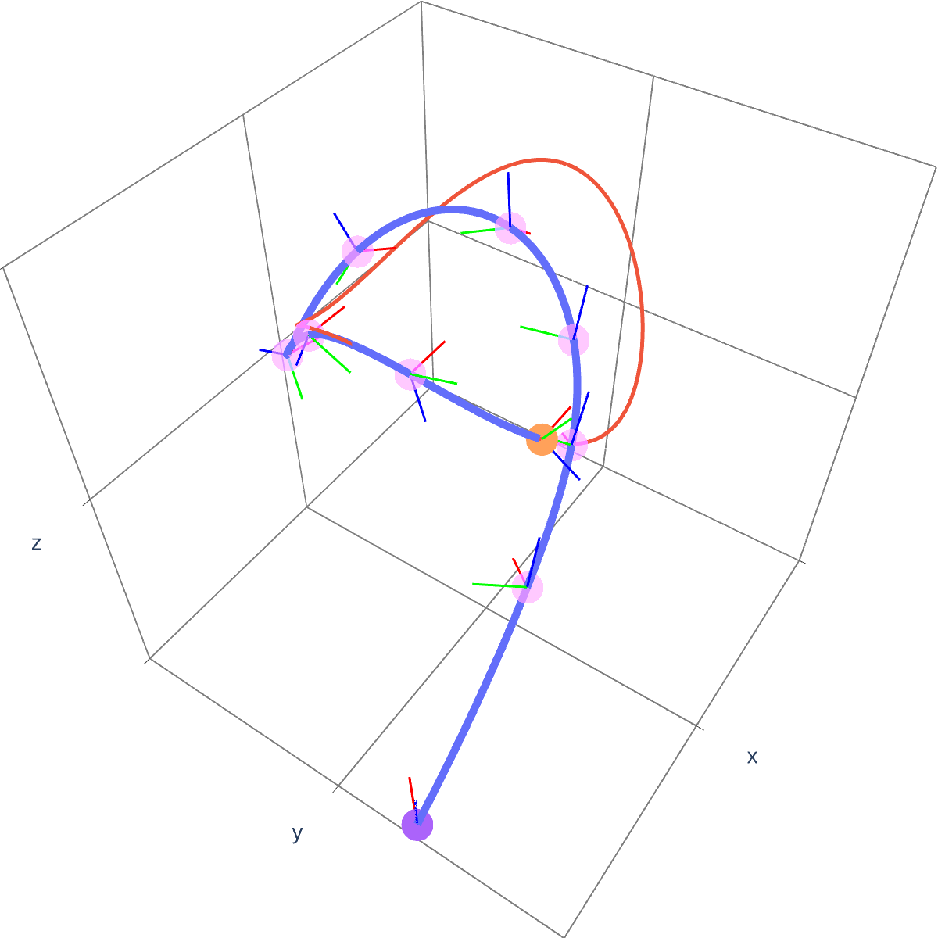
\includegraphics[width=\textwidth]{figures/vf_automatica_1.pdf} % Replace with your image
        \caption{$t\in[0, 5]s$}
        \label{fig:vfplot-first}
    \end{subfigure}
    \hfill
    % Second subfigure
    \begin{subfigure}[b]{0.32\textwidth}
        \centering
        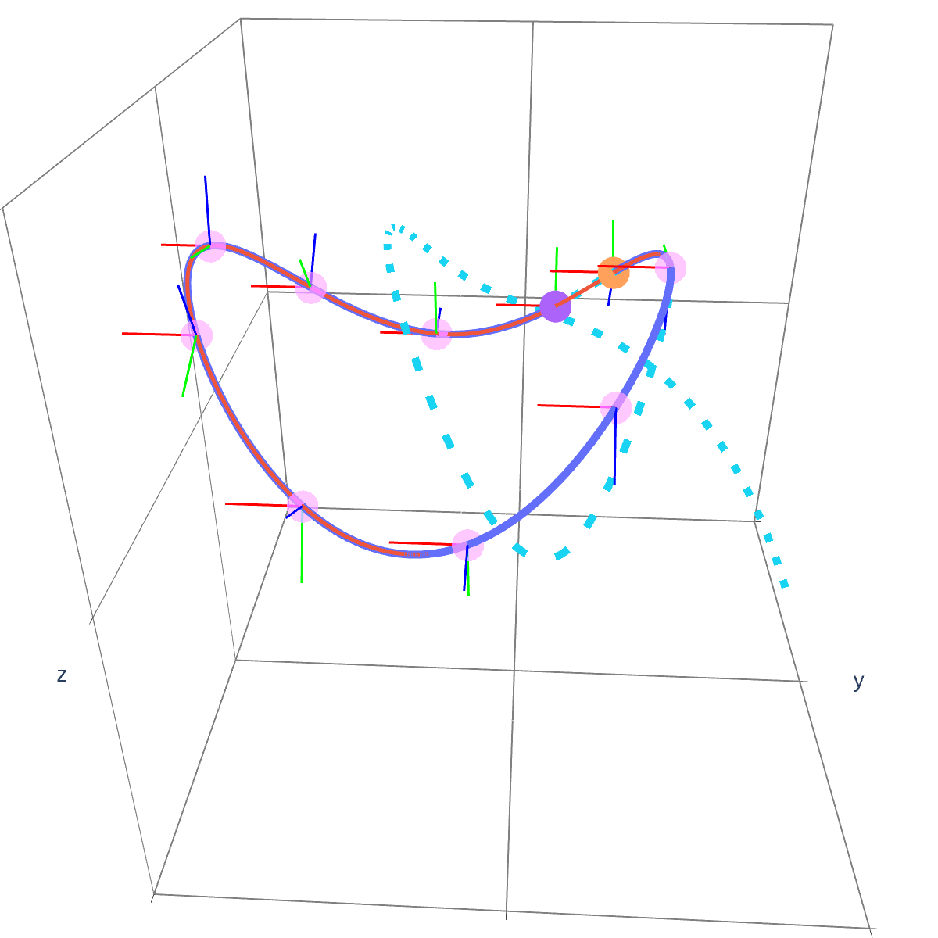
\includegraphics[width=\textwidth]{figures/vf_automatica_2.pdf} % Replace with your image
        \caption{$t\in[5, 9.7]s$}
        \label{fig:vfplot-second}
    \end{subfigure}
    \hfill
    % Third subfigure
    \begin{subfigure}[b]{0.32\textwidth}
        \centering
        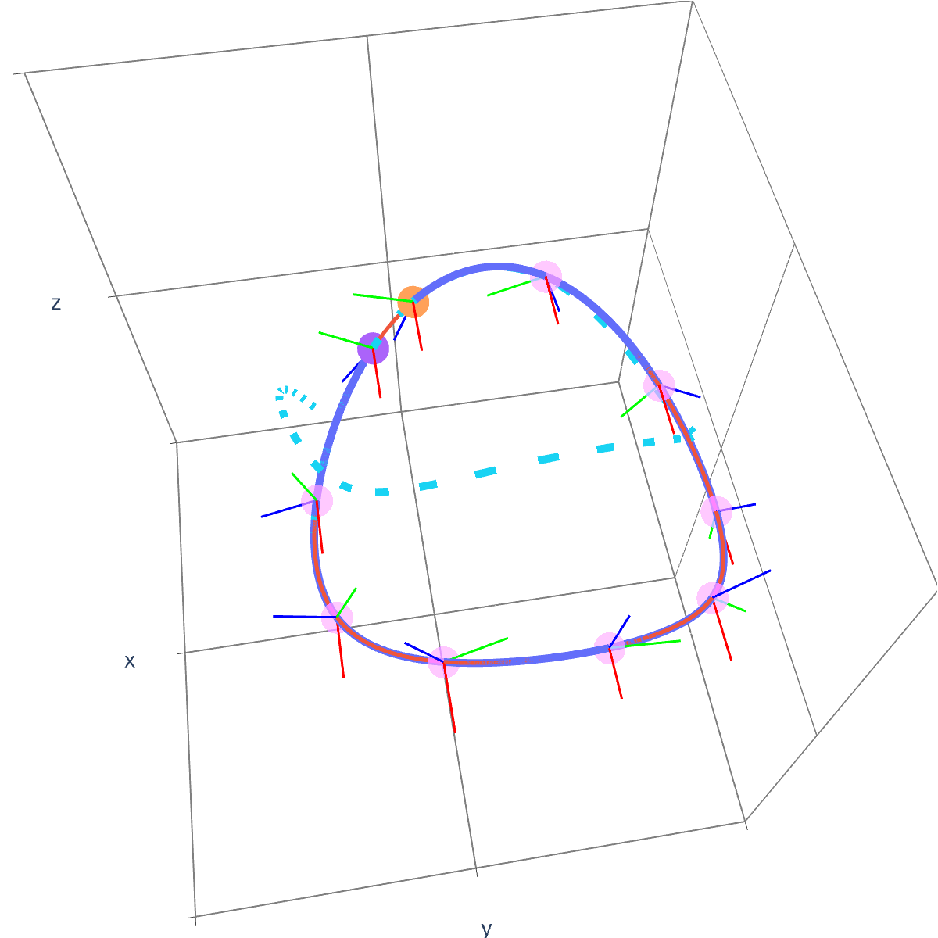
\includegraphics[width=\textwidth]{figures/vf_automatica_3.pdf} % Replace with your image
        \caption{$t\in[9.7, 14.5]s$}
        \label{fig:vfplot-third}
    \end{subfigure}
    \caption{The solid blue line depicts the system trajectory, while the solid red line indicates the target curve. The dashed light blue line represents the past trajectory. The initial and final positions are marked by purple and orange spheres, respectively. Translucent pink spheres denote intermediary positions, with orientation frames shown by RGB axes.}
    \label{fig:vfplot-trajectory}
\end{figure}
\begin{figure}[ht!]
    \centering
    \def\svgwidth{.8\linewidth}
    {\tiny\import{figures/}{distance_pos_ori_D.pdf_tex}}
    \caption{Value of EC-distance $D$, position error in centimeters and orientation error in degrees along time.}
    \label{fig:position-orientation-errors}
\end{figure}
We implemented the code in C++. On average, the computation of the vector field took $60\pm5$ milliseconds per iteration on a single core of an Intel i5-10300H @ 4.5GHz CPU, with 8 GB of RAM. On average, $99.5\%$ of this time was spent solving the optimization problem in \eqref{eq:optimization-problem-distance-definition-point-curve}. Since the optimization process is highly parallelizable -- allowing for the simultaneous computation of $\widehat{D}(\mathbf{H},\mathbf{H}_d(s))$ across different discretized $s$ -- the computational effort could be significantly reduced by leveraging parallel architectures such as GPUs, SIMD, or multi-threading. The system's trajectory is illustrated in \cref{fig:vfplot-trajectory}, while the values of the distance function $D$ are shown in \cref{fig:position-orientation-errors}. Additionally, \cref{fig:position-orientation-errors} provides a more intuitive representation of the position error (in centimeters) and the orientation error (in degrees). The results confirm that the system successfully converges to the desired curve and circulates around it as expected. Once the system reaches the curve, it remains there without deviation. Although our implementation was carried out in C++, we provide a less efficient sample code in Python for clarity and accessibility, available at \url{https://github.com/fbartelt/SE3-example/blob/main/SE3example.ipynb}.

\section{Collaborative Manipulation}
For the conduction of the adaptive control simulation of \cref{ch:collaborative}, we considered the manipulation of a large cylindrical body by six agents, aiming to converge to and circulate a curve $\mathcal{C}\in\text{ISE}(3)$. The cylindrical body had a radius $r$ of $\qty{0.25}{\meter}$, a height $h$ of $\qty{1}{\meter}$ and a mass $m$ of $\qty{1.28E3}{\kilogram}$. The measurement point $\mathbf{r}_p$ was taken as the position of the first agent $\mathbf{r}_1=[0\ 0\ 1.5]^\top$. The other agents' positions as well as the inertia tensor components are detailed in \cref{tb:parameters}.
\begin{table}[htb]
    \centering
    \begin{threeparttable}
    \caption{Adaptive simulation parameters}\label{tb:parameters}
    \begin{tabular}{clcl}
    Parameter & Value & Parameter & Value\\\hline
    $r$ & $\qty{0.25}{\meter}$ & $\mathbf{r}_{1}$ & $[0\ 0\ 1.5]^\top\,\unit{\meter}$\\
    $h$ & $\qty{1}{\meter}$ & $\mathbf{r}_{2}$ & $[0\ 0\ -1.5]^\top\,\unit{\meter}$\\
    $m$ & $\qty{1.28E3}{\kilogram}$ & 
    $\mathbf{r}_{3}$ & $[0.5\ 0\ 0]^\top\,\unit{\meter}$\\
    $\mathbb{I}_{\text{cm}, xx}$ & $\qty{1.56E2}{\kilogram\meter\squared}$ & 
    $\mathbf{r}_{4}$ & $[-0.5\ 0\ 0]^\top\,\unit{\meter}$\\  
    $\mathbb{I}_{\text{cm}, yy}$ & $\qty{1.56E2}{\kilogram\meter\squared}$ &
    $\mathbf{r}_{5}$ & $[0\ 0.5\ 0]^\top\,\unit{\meter}$\\
    $\mathbb{I}_{\text{cm}, zz}$ & $\qty{4.93E1}{\kilogram\meter\squared}$  & 
    $\mathbf{r}_{6}$ & $[0\ -0.5 \ 0]^\top\,\unit{\meter}$\\
    $\mathbf{r}_{p}$ & $[0\ 0\ 1.5]^\top\,\unit{\meter}$ \\\hline
    \end{tabular}
    \begin{tablenotes}
        \footnotesize
        \item Note: The inertia tensor $\mathbb{I}_\text{cm}$ is a diagonal matrix for which the components $\mathbb{I}_{\text{cm}, xx}, \mathbb{I}_{\text{cm}, yy}$ and $\mathbb{I}_{\text{cm}, zz}$ are the diagonal elements in order.
    \end{tablenotes}
    \end{threeparttable}
\end{table}

The curve constants were set to $c_1 = 0.7$ and $c_2 = 0.4$, and $s$ was discretized into $5000$ evenly spaced samples within the interval $[0, 1]$, thus $\Delta s=1\slash5000$. For function $H$ we set $\kappa=1.4$. . The agents were symmetrically distributed, and the measurement point was located at the position of the first agent. Additionally, the dead zone strategy \citep{ioannou2012robust} was employed for $\|\boldsymbol{\zeta}\| \le 0.01$, in which no adaptation will occur.

\subsection{Curve parametrization}
In this simulation, we employed a more complex curve in the group $\text{ISE}(3)$, which was defined as
\begin{align}
    \mathbf{H}_d(s) = \begin{bmatrix}
        \mathbf{R}_d(s) & \mathbf{0} & \mathbf{0}\\
        \mathbf{0} & \mathbf{I} & \mathbf{p}_d(s)\\
        \mathbf{0} & \mathbf{0} & 1
    \end{bmatrix},\label{eq:parametriceq-simulation}
\end{align}
where
\begin{align}
    \mathbf{p}_d(s) &= \begin{bmatrix}
        0.7(\sin(2\pi s) + 2\sin(4\pi s))\\
        0.7(\cos(2\pi s) - 2\cos(4\pi s))\\
        0.4 - 0.7\sin(6\pi s)
    \end{bmatrix},\\
    \mathbf{R}_d(s) &= \begin{bmatrix}
        \cos(2\pi s) & -\sin(2\pi s) & 0\\
        \sin(2\pi s) & \cos(2\pi s) & 0\\
        0 & 0 & 1
    \end{bmatrix}\begin{bmatrix}
        1 & 0 & 0\\
        0 & \cos(4\pi s) & -\sin(4\pi s)\\
        0 & \sin(4\pi s) & \cos(4\pi s)
    \end{bmatrix}.
\end{align}
Instead of using the continuous curve, we discretized it into $P=\num{2000}$ points by sampling $s$ into $\num{2000}$ evenly spaced points within the interval $[0, 1]$. In order to distinguish both, we henceforth adopt the notations $\mathbf{H}_d[i]$, $\mathbf{p}_d[i]$ and $\mathbf{R}_d[i]$ to refer to the $i$-th sample of the curve, position and orientation, respectively.


In both simulations, we employed the forward Euler method with a time step of $\Delta t = \qty{1E-2}{\second}$. 
\subsection{Employed nummerical methods}\label{sec:results-adaptive-nummerical-methods}
Although the curve has a representation in $\text{ISE}(3)$, our adaptive control formulation was based on the tuple representation of $\mathbb{R}^3\times \text{SO}(3)$, thus, to distinguish both, in this section we use the notation $\mathbf{H}$ to represent the element of $\text{ISE}(3)$ and $\boldsymbol{\chi}=(\mathbf{R}, \mathbf{p})$ to represent the same entity as an element of $\mathbb{R}^3\times \text{SO}(3)$. This equivalence also implies that $\boldsymbol{\xi}=\dot{\boldsymbol{\chi}}$ and $\dot{\boldsymbol{\xi}} = \ddot{\boldsymbol{\chi}}$, thus we adopt the notation using $\boldsymbol{\chi}$ for twists and accelerations to maintain consistency with the dynamics in \cref{sec:dynamic-modelling}.

The first consideration needed is about the reference model. As defined in \eqref{eq:ref-model-linear-parametrization}, the reference model depends on an acceleration given by the derivative of the vector field. This was approximated by the symmetric difference quotient:
\begin{align}
    \dot{\Psi}\bigl(\mathbf{H}(t)\bigr) \approx \frac{\Psi\Biggl(\exp\biggl(\SL\Bigl(\Delta t\Psi\bigl(\mathbf{H}(t)\bigr)\Bigr)\biggr)\mathbf{H}(t)\Biggr) - \Psi\Biggl(\exp\biggl(\SL\Bigl(-\Delta t\Psi\bigl(\mathbf{H}(t)\bigr)\Bigr)\biggr)\mathbf{H}(t)\Biggr)}{2\Delta t}. \label{eq:approximation-derivative-psi}
\end{align}
With this, we can start discussing the integration of the system. We utilized the \emph{Heun's method} \citep[p. 330]{fred2007algoritmos}, also known as the \emph{improved Euler method}, which is a two-stage Runge-Kutta method. To describe how this method was applied in the context of Lie groups, we will use the notation $\underline{\cdot}$ to denote the intermediate variables in the Heun's method. Adopting $\mathbf{H}_\text{ref}$ as the reference state, i.e., the state of the original system if it were following the vector field perfectly, the update of the system's acceleration $\ddot{\boldsymbol{\chi}}$, parameters derivative $\dot{\widehat{\mathbf{o}}}_i$ and $\dot{\widehat{\mathbf{r}}}_i$, and the respective intermediary variables were taken as follows:
\begin{align}
    \begin{split}
        \ddot{\underline{\boldsymbol{\chi}}}(t+\Delta t) &= \mathbf{M}\bigl(\underline{\boldsymbol{\chi}}(t)\bigr)^{\dagger(\epsilon)}\biggl(-\mathbf{C}\bigl(\underline{\boldsymbol{\chi}}(t), \underline{\dot{\boldsymbol{\chi}}}(t)\bigr)\underline{\dot{\boldsymbol{\chi}}}(t)  + \sum_{i=1}^6 \mathbf{G}\bigl(\underline{\boldsymbol{\chi}}(t), \underline{\widehat{\mathbf{r}}}_i(t)\bigr)^{-1}\underline{\boldsymbol{\eta}}_i(t)\biggr)\\
        \ddot{{\boldsymbol{\chi}}}(t+\Delta t) &= \mathbf{M}\bigl({\boldsymbol{\chi}}(t)\bigr)^{\dagger(\epsilon)}\biggl(-\mathbf{C}\bigl({\boldsymbol{\chi}}(t), {\dot{\boldsymbol{\chi}}}(t)\bigr)\dot{\boldsymbol{\chi}}(t)  + \sum_{i=1}^6 \mathbf{G}\bigl({\boldsymbol{\chi}}(t), {\widehat{\mathbf{r}}}_i(t)\bigr)^{-1}{\boldsymbol{\eta}}_i(t)\biggr)\\
        \underline{\dot{\widehat{\mathbf{o}}}}_i(t + \Delta t) &= -\boldsymbol{\Gamma}_o\mathbf{Y}_o\Bigl(\underline{\boldsymbol{\chi}}(t), \underline{\dot{\boldsymbol{\chi}}}(t), \Psi\bigl(\underline{\mathbf{H}}_\text{ref}(t)\bigr), \dot{\Psi}\bigl(\underline{\mathbf{H}}_\text{ref}(t)\bigr)\Bigr)\underline{\boldsymbol{\zeta}}\\
        {\dot{\widehat{\mathbf{o}}}}_i(t + \Delta t) &= -\boldsymbol{\Gamma}_o\mathbf{Y}_o\Bigl({\boldsymbol{\chi}}(t), {\dot{\boldsymbol{\chi}}}(t), \Psi\bigl({\mathbf{H}_\text{ref}}(t)\bigr), \dot{\Psi}\bigl({\mathbf{H}_\text{ref}}(t)\bigr)\Bigr){\boldsymbol{\zeta}}\\
        \underline{\dot{\widehat{\mathbf{r}}}}_i(t + \Delta t) &= -\boldsymbol{\Gamma}_r\mathbf{Y}_r\bigl(\underline{\boldsymbol{\eta}}_i(t), \underline{\boldsymbol{\chi}}(t)\bigr)\underline{\boldsymbol{\zeta}}\\
        \underline{\dot{\widehat{\mathbf{r}}}}_i(t + \Delta t) &= -\boldsymbol{\Gamma}_r\mathbf{Y}_r\bigl({\boldsymbol{\eta}}_i(t), {\boldsymbol{\chi}}(t)\bigr){\boldsymbol{\zeta}},
    \end{split}
\end{align}
where $\underline{\boldsymbol{\eta}}_i(t) = \mathbf{Y}_o\Bigl(\underline{\boldsymbol{\chi}}(t), \underline{\dot{\boldsymbol{\chi}}}(t), \Psi\bigl(\underline{\mathbf{H}}_\text{ref}(t)\bigr), \dot{\Psi}\bigl(\underline{\mathbf{H}}_\text{ref}(t)\bigr)\Bigr)\underline{\widehat{\mathbf{o}}}_i(t) - \mathbf{K}_D\underline{\boldsymbol{\zeta}}$, the intermediary velocity error $\underline{\boldsymbol{\zeta}}=\underline{\dot{\boldsymbol{\chi}}}(t) - \Psi\bigl(\underline{\mathbf{H}}_\text{ref}(t)\bigr)$, and $\mathbf{M}^{\dagger(\epsilon)}$ is the damped pseudo inverse $\mathbf{M}^{\dagger(\epsilon)} = (\mathbf{M}^\top\mathbf{M} + \epsilon\mathbf{I})^{-1}\mathbf{M}^\top$, with $\epsilon=0.01$. The update of the system's twist and parameters estimates were given by
\begin{align}
    \begin{split}
        \underline{\dot{\boldsymbol{\chi}}}(t + \Delta t) &= \dot{\boldsymbol{\chi}}(t) + \Delta t \ddot{\underline{\boldsymbol{\chi}}}(t)\\
        \dot{\boldsymbol{\chi}}(t + \Delta t) &= \dot{\boldsymbol{\chi}}(t) + \frac{\Delta t}{2} \bigl(\ddot{\boldsymbol{\chi}}(t) + \underline{\ddot{\boldsymbol{\chi}}}(t)\bigr)\\
        \widehat{\mathbf{o}}_i(t + \Delta t) &= \widehat{\mathbf{o}}_i(t) + \frac{\Delta t}{2} \bigl(\dot{\widehat{\mathbf{o}}}_i(t) + \underline{\dot{\widehat{\mathbf{o}}}}_i(t)\bigr)\\
        \widehat{\mathbf{r}}_i(t + \Delta t) &= \widehat{\mathbf{r}}_i(t) + \frac{\Delta t}{2} \bigl(\dot{\widehat{\mathbf{r}}}_i(t) + \underline{\dot{\widehat{\mathbf{r}}}}_i(t)\bigr).
    \end{split}
\end{align}
The update of the system's state was given by
\begin{align}
    \begin{split}
        \underline{\mathbf{H}}(t +\Delta t) &= \exp\Bigl(\Delta t\SL\bigl(\dot{\boldsymbol{\chi}}(t)\bigr)\Bigr)\mathbf{H}(t)\\
        \mathbf{H}(t + \Delta t) &= \exp\biggl(\frac{\Delta t}{2}\SL[\dot{\boldsymbol{\chi}}(t) + \underline{\dot{\boldsymbol{\chi}}}(t)]\biggr)\mathbf{H}(t)\\
        \underline{\mathbf{H}}_\text{ref}(t +\Delta t) &= \exp\biggl(\Delta t\SL\Bigl(\Psi\bigl(\mathbf{H}(t)\bigr)\Bigr)\biggr)\mathbf{H}(t)\\
        \mathbf{H}_\text{ref} (t + \Delta t) &= \mathbf{H}(t + \Delta t)
    \end{split}
\end{align}

As defined in \cref{sec:collaborative-path-planning}, the normal component is discontinuous. In order to avoid chattering and noise propagation due to the nummerical dofferentiations, we employed a smoothing strategy to the distance function $D$. The smoothed distance $\bar{D}$ is defined in terms of the discretized curve as
\begin{align}
    \bar{D}(\mathbf{H}) = D(\mathbf{H}) - \delta\log\biggl(\frac{\sum_{i=1}^{P}w_i}{P}\biggr),
\end{align}
where $\delta=0.05$ is a smoothing factor, $P=\num{2000}$ is the total number of points in the curve, and $w_i$ are the distance weights defined as
\begin{align}
    w_i = \frac{\exp\bigl(D(\mathbf{H}) - \widehat{D}(\mathbf{H}, \mathbf{H}_d[i])\bigr)}{\delta}.
\end{align}
With this, the $\text{L}$ operator of the smoothed distance is given as
\begin{align}
    \text{L}[\bar{D}](\mathbf{H}) = \frac{\sum_{i=1}^{P}w_i\text{L}_\mathbf{V}[\widehat{D}]\bigl(\mathbf{H}, \mathbf{H}_d[i]\bigr)}{\sum_{i=1}^{P}w_i},
\end{align}
which implies that the $j^{th}$ entry of the normal component $\boldsymbol{\xi}_{N,j}$ can be approximated as
\begin{align}
    \boldsymbol{\xi}_{N,j}(\mathbf{H}) = -\frac{\sum_{i=1}^{P} \frac{w_i}{\varepsilon}\biggl(\widehat{D}\Bigl(\exp\bigl(\varepsilon\SL[\mathbf{e}_j]\bigr)\mathbf{H}, \mathbf{H}_d[i]\Bigr)- \widehat{D}\bigl(\mathbf{H}, \mathbf{H}_d[i]\bigr)\biggr)}{\sum_{i=1}^{P}w_i}
\end{align}
with $\varepsilon=0.001$.

As the curve parametrization has an explicit equation \cref{eq:parametriceq-simulation}, the derivative $\frac{d}{ds}\mathbf{H}_d(s)$ was computed analytically. Thus, the derivative of the $i^{th}$ point in the discretized curve is given by $\mathbf{H}_d'[i]$. The smoothed tangent component $\boldsymbol{\xi}_T$ is then expressed as
\begin{align}
    \boldsymbol{\xi}_T(\mathbf{H}) = \frac{\sum_{i=1}^{P} w_i\invSL\bigl(\mathbf{H}_d'[i]\mathbf{H}_d[i]^{-1}\bigr)}{\sum_{i=1}^{P} w_i}
\end{align}

This smoothing process behaves as an interpolation to determine the nearest point, as such it deforms the original curve to an interpolated one. The parameter $\delta$ weights this deformation. Although this strategy prevents us from invoking the already proven lemmas and theorems, we claim that all signals will remain bounded and the system will converge to a neighborhood of the curve that is sufficiently close for the task.

The computation of the real distance $D(\mathbf{H})$ was performed through a brute force approach using a slight modification of the expression derived in \cref{sec:collaborative-ee-distance-computation}. To avoid nummerical errors, the distance was computed as
\begin{align}
    D(\mathbf{H}) = \sqrt{2\theta^2 + \|\mathbf{u}\|^2 + 0.01^2} - 0.01
\end{align}

\subsection{Controller parameters}
As we use the vector field strategy as a reference to the adaptive control, we need to specify the vector field gains. The gains $k_N(\mathbf{H})$ and $k_T(\mathbf{H})$ were defined as
\begin{align}
    k_N(\mathbf{H}) &= \tanh\Bigl(10\bigl(\bar{D}(\mathbf{H})- \gamma\bigr)\Bigr),\\
    k_T(\mathbf{H}) &= 0.2\Bigl(1 - \tanh\bigl(\bar{D}(\mathbf{H}) - \gamma\bigr)\Bigr),
\end{align}
where $\gamma=0.27$ is an offset determined by evaluating the offset between the smoothed distance $\bar{D}$ and the real distance $D$ in steady state.

As for the adaptive control, the adaptation gains were set as
\begin{align}
    \boldsymbol{\Gamma}_o &= \frac{1}{30}\diag\bigl(\abs(\mathbf{o}_i) + \num{1E-2}\bigr)\\
    \boldsymbol{\Gamma}_r &= \frac{1}{3000}\mathbf{I}_{3\times3},
\end{align}
where $\diag(\cdot)$ maps a vector into a diagonal matrix, and $\abs(\cdot)$ is the element-wise absolute value of a vector. The control gain was defined as
\begin{align}
    \mathbf{K}_D = 3.5\blkdiag\bigl(\num{20E3}\mathbf{I}_{3\times3},\, \num{25E3}\mathbf{I}_{3\times3}\bigr),
\end{align}
where $\blkdiag(\cdot,\, \dots,\, \cdot)$ maps a list of matrices into a block diagonal matrix.
\subsection{Simulation}
The simulation was conducted for $\qty{40}{\second}$ and a time step was $\Delta t=\num{1E3}$ for the integration described in \cref{sec:results-adaptive-nummerical-methods}. The dead zone strategy (see \cref{sec:background-adaptive-control}) was employed adopting a deadband $\|\boldsymbol{\zeta}\| \le 0.01$. The initial conditions were set as follows:
\begin{align}
    \mathbf{p}(0) &= \begin{bmatrix}
        -0.1 & 0 & 0.2
    \end{bmatrix}^\top\\
    \mathbf{R}(0) &= \begin{bmatrix}
        \cos\bigl(\frac{\pi}{4}\bigr) & -\sin\bigl(\frac{\pi}{4}\bigr) & 0\\
        \sin\bigl(\frac{\pi}{4}\bigr) & \cos\bigl(\frac{\pi}{4}\bigr) & 0\\
        0 & 0 & 1
    \end{bmatrix}.
\end{align}

The initial estimates $\widehat{\mathbf{o}}_i$ and $\widehat{\mathbf{r}}_i$ were randomly initialized with a normal distribution having zero mean and standard deviations of $1$ and $2$, respectively. 
\begin{figure}[ht]
    \centering
    % First subfigure
    \begin{subfigure}[b]{0.32\textwidth}
        \centering
        \def\svgwidth{\linewidth}
        {\import{figures/}{adaptive_traj1.pdf_tex}}
        \caption{$t\in[0, 13]s$}
        \label{fig:adaptive-traj-first}
    \end{subfigure}
    \hfill
    % Second subfigure
    \begin{subfigure}[b]{0.32\textwidth}
        \centering
        \def\svgwidth{\linewidth}
        {\import{figures/}{adaptive_traj2.pdf_tex}}
        \caption{$t\in[13, 26]s$}
        \label{fig:adaptive-traj-second}
    \end{subfigure}
    \hfill
    % Third subfigure
    \begin{subfigure}[b]{0.32\textwidth}
        \centering
        \def\svgwidth{\linewidth}
        {\import{figures/}{adaptive_traj3.pdf_tex}}
        \caption{$t\in[26, 39]s$}
        \label{fig:adaptive-traj-third}
    \end{subfigure}
    \caption{Trajectory of the manipulated cylinder. The solid blue line depicts the system trajectory, while the solid red line indicates the target curve. The dashed light blue line represents the past trajectory. The initial and final positions are marked by purple and orange cylinders, respectively. Pink cylinders denote intermediary positions, with orientation frames shown by RGB axes.}
    \label{fig:adaptive-trajectory}
\end{figure}

The trajectory of the manipulated object is shown in \cref{fig:adaptive-trajectory}. The figure shows three different perspectives to facilitate the target curve, depicted in red, visualization. The trajectory of the system is shown in blue and divided into three time segments, $t\in[0,\,13]s$, $t\in[13,\,26]s$ and $t\in[26,\,39]s$. In each segment, eight cylinders are shown to represent the object's movement during the simulation, as well as its orientation frames. As can be seen, the object rapidly converges to the curve and follows it closely.

\begin{figure}[ht]
    \centering
    \def\svgwidth{\linewidth}
    {\footnotesize\import{figures/}{adaptive_snorm.pdf_tex}}
    \caption{Norm of error vector $\boldsymbol{\zeta}$ during the adaptive control simulation.}
    \label{fig:sim2-snorm}
\end{figure}
The error vector $\boldsymbol{\zeta}$ rapidly decreased to zero, however after $\qty{0.8}{\second}$ it increases slightly, as shown in \cref{fig:sim2-snorm}. This behavior is expected due to the adaptation process. After approximately $\qty{1.2}{\second}$, $\boldsymbol{\zeta}$ converged to $\num{0.01}$, indicating that the agents successfully track the desired velocity, the vector field. The norm of this error exhibits some oscillations for the rest of the simulation, but it remains close to zero. These oscillations can be explained through the dead-zone strategy and the approximations made in the computations.

\begin{figure}[ht]
    \centering
    \def\svgwidth{\linewidth}
    {\footnotesize\import{figures/}{adaptive_distances.pdf_tex}}
    \caption{Distance $D$ during adaptive control simulation, along with the position error in centimeters and orientation error in degrees.}
    \label{fig:sim2-distances}
\end{figure}
Observing the behavior of the distance function $D$ in \cref{fig:sim2-distances}, we can see that the object approached the curve asymptotically at around $\qty{1.2}{\second}$, as expected from the behavior of $\boldsymbol{\zeta}$. The final value observed for $D$ is $\num{0.004}$, which translates to a position error of $\qty{0.6}{\centi\meter}$ and an orientation error of $\qty{0.32}{\degree}$.

The average forces and torques applied by each agent are shown in \cref{tb:forces} and \cref{tb:torques}, respectively. The average force and standard deviation were similar to each agent and were approximately $\qty{88 \pm 111}{\newton}$. The maximum and minimum force were also similar and approximately $\qty{7411}{\newton}$ and $\qty{31}{\newton}$, respectively. The torques applied by each agent were more varied, with the highest average observed for agent $5$ at $\qty{392.079 \pm 573.948}{\newton\meter}$ and the lowest for agent $3$ at $\qty{109.546 \pm 138.17}{\newton\meter}$. The maximum torque was $\qty{46835.582}{\newton\meter}$, applied by agent $5$, and the minimum was $\qty{3.731}{\newton\meter}$, applied by agent $2$. These high values are expected, since the cylinder has a large mass and dimensions, and the agents perform a complex manipulation task in minimum time. The maximum linear speed experienced by the object was $\qty{1.09}{\meter\per\second}$, and the maximum angular velocity was $\qty{1.04}{\radian\per\second}$, which are quite demanding values.
\begin{table}[ht]
    \centering
    \caption{Statistics of the forces applied by each agent}\label{tb:forces}
    \begin{tabular}{clll}
    Agent & Average Force & Min. Force & Max. Force\\\hline
    $1$ & $\qty{88.093 \pm 111.561}{\newton}$ & $\qty{30.833}{\newton}$ & $\qty{7411.424}{\newton}$ \\
    $2$ & $\qty{88.159 \pm 111.621}{\newton}$ & $\qty{31.208}{\newton}$ & $\qty{7411.544}{\newton}$ \\
    $3$ & $\qty{88.562 \pm 111.718}{\newton}$ & $\qty{31.150}{\newton}$ & $\qty{7411.903}{\newton}$ \\
    $4$ & $\qty{88.015 \pm 111.579}{\newton}$ & $\qty{31.151}{\newton}$ & $\qty{7410.960}{\newton}$ \\
    $5$ & $\qty{88.395 \pm 111.689}{\newton}$ & $\qty{31.204}{\newton}$ & $\qty{7411.755}{\newton}$ \\
    $6$ & $\qty{87.703 \pm 111.502}{\newton}$ & $\qty{31.017}{\newton}$ & $\qty{7411.278}{\newton}$
    \\\hline
    \end{tabular}
\end{table}
\begin{table}[ht]
    \centering
    \caption{Statistics of the torques applied by each agent}\label{tb:torques}
    \begin{tabular}{clll}
    Agent & Average Torque & Min. Torque & Max. Torque\\\hline
    $1$ & $\qty{148.854 \pm 181.826}{\newton\meter}$ & $\qty{54.256}{\newton\meter}$ & $\qty{8737.108}{\newton\meter}$\\
    $2$ & $\qty{114.282 \pm 139.403}{\newton\meter}$ & $\qty{3.731}{\newton\meter}$ & $\qty{4838.576}{\newton\meter}$\\
    $3$ & $\qty{109.546 \pm 138.178}{\newton\meter}$ & $\qty{6.095}{\newton\meter}$ & $\qty{8539.131}{\newton\meter}$\\
    $4$ & $\qty{253.599 \pm 288.916}{\newton\meter}$ & $\qty{79.889}{\newton\meter}$ & $\qty{15571.921}{\newton\meter}$\\
    $5$ & $\qty{392.079 \pm 573.948}{\newton\meter}$ & $\qty{48.958}{\newton\meter}$ & $\qty{46835.582}{\newton\meter}$\\
    $6$ & $\qty{145.025 \pm 207.934}{\newton\meter}$ & $\qty{42.274}{\newton\meter}$ & $\qty{12251.425}{\newton\meter}$
    \\\hline
    \end{tabular}
\end{table}